\documentclass[aspectratio=169]{beamer}

% === Theme Configuration ===
\usetheme{Madrid}
\usecolortheme{whale}
\setbeamertemplate{navigation symbols}{}
\setbeamertemplate{footline}[frame number]

% === Packages ===
\usepackage[utf8]{inputenc}
\usepackage[romanian]{babel}
\usepackage{amsmath,amsfonts,amssymb}
\usepackage{graphicx}
\usepackage{listings}
\usepackage{xcolor}
\usepackage{tikz}
\usetikzlibrary{shapes,arrows,positioning,calc}
\usepackage{hyperref}
\usepackage{booktabs}
\usepackage{multicol}

% === Colors ===
\definecolor{codegreen}{rgb}{0,0.6,0}
\definecolor{codegray}{rgb}{0.5,0.5,0.5}
\definecolor{codepurple}{rgb}{0.58,0,0.82}
\definecolor{backcolour}{rgb}{0.95,0.95,0.92}
\definecolor{primaryblue}{RGB}{99,102,241}
\definecolor{accentorange}{RGB}{245,158,11}

% === Code Listings ===
\lstdefinestyle{gostyle}{
    backgroundcolor=\color{backcolour},
    commentstyle=\color{codegreen},
    keywordstyle=\color{magenta},
    numberstyle=\tiny\color{codegray},
    stringstyle=\color{codepurple},
    basicstyle=\ttfamily\scriptsize,
    breakatwhitespace=false,
    breaklines=true,
    captionpos=b,
    keepspaces=true,
    numbers=left,
    numbersep=5pt,
    showspaces=false,
    showstringspaces=false,
    showtabs=false,
    tabsize=2
}
\lstset{style=gostyle}

% === Title Information ===
\title[Proiect Criptografie]{Securitate Criptografică}
\subtitle{One-Time Pad și Algoritmi Criptografici Moderni}
\author{Proiect de Criptografie}
\institute{Facultatea de Informatică}
\date{\today}

\begin{document}

% === Title Slide ===
\begin{frame}
    \titlepage
\end{frame}

% === Outline ===
\begin{frame}{Cuprins}
    \tableofcontents
\end{frame}

% ============================================================
\section{Introducere în Criptografie}
% ============================================================

\begin{frame}{Ce este Criptografia?}
    \begin{columns}
        \begin{column}{0.5\textwidth}
            \textbf{Definiție:}
            \begin{itemize}
                \item Știința comunicării secrete
                \item Transformarea informației pentru protecție
                \item Asigurarea confidențialității, integrității și autenticității
            \end{itemize}

            \vspace{0.5cm}
            \textbf{Terminologie:}
            \begin{itemize}
                \item \textbf{Plaintext} (M) - mesaj original
                \item \textbf{Ciphertext} (C) - mesaj criptat
                \item \textbf{Key} (K) - cheie secretă
                \item \textbf{Encryption} - criptare: $E_K(M) = C$
                \item \textbf{Decryption} - decriptare: $D_K(C) = M$
            \end{itemize}
        \end{column}
        \begin{column}{0.5\textwidth}
            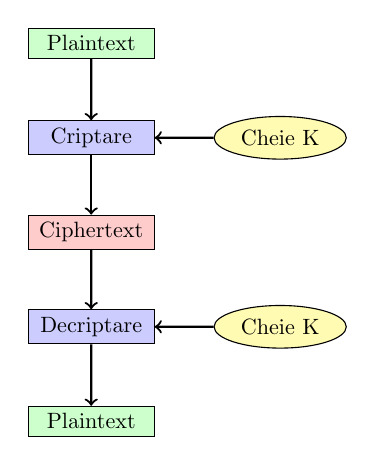
\begin{tikzpicture}[node distance=1.5cm, auto, scale=0.8, transform shape]
                \node[draw, rectangle, fill=green!20, minimum width=2cm] (plain) {Plaintext};
                \node[draw, rectangle, fill=blue!20, minimum width=2cm, below of=plain] (enc) {Criptare};
                \node[draw, rectangle, fill=red!20, minimum width=2cm, below of=enc] (cipher) {Ciphertext};
                \node[draw, rectangle, fill=blue!20, minimum width=2cm, below of=cipher] (dec) {Decriptare};
                \node[draw, rectangle, fill=green!20, minimum width=2cm, below of=dec] (plain2) {Plaintext};
                \node[draw, ellipse, fill=yellow!30, right of=enc, xshift=1.5cm] (key1) {Cheie K};
                \node[draw, ellipse, fill=yellow!30, right of=dec, xshift=1.5cm] (key2) {Cheie K};

                \draw[->, thick] (plain) -- (enc);
                \draw[->, thick] (enc) -- (cipher);
                \draw[->, thick] (cipher) -- (dec);
                \draw[->, thick] (dec) -- (plain2);
                \draw[->, thick] (key1) -- (enc);
                \draw[->, thick] (key2) -- (dec);
            \end{tikzpicture}
        \end{column}
    \end{columns}
\end{frame}

\begin{frame}{Clasificarea Algoritmilor Criptografici}
    \begin{center}
        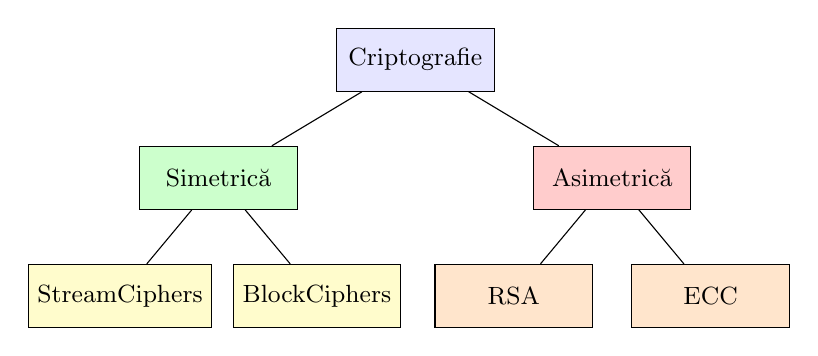
\begin{tikzpicture}[
            level 1/.style={sibling distance=5cm},
            level 2/.style={sibling distance=2.5cm},
            every node/.style={rectangle, draw, fill=blue!10, minimum width=2cm, minimum height=0.8cm, font=\small}
        ]
            \node {Criptografie}
                child {node[fill=green!20] {Simetrică}
                    child {node[fill=yellow!20] {Stream\\Ciphers}}
                    child {node[fill=yellow!20] {Block\\Ciphers}}
                }
                child {node[fill=red!20] {Asimetrică}
                    child {node[fill=orange!20] {RSA}}
                    child {node[fill=orange!20] {ECC}}
                };
        \end{tikzpicture}
    \end{center}

    \vspace{0.5cm}
    \begin{columns}
        \begin{column}{0.5\textwidth}
            \textbf{Criptare Simetrică:}
            \begin{itemize}
                \item Aceeași cheie pentru criptare/decriptare
                \item Rapidă și eficientă
                \item Exemple: AES, OTP, DES
            \end{itemize}
        \end{column}
        \begin{column}{0.5\textwidth}
            \textbf{Criptare Asimetrică:}
            \begin{itemize}
                \item Chei diferite (publică/privată)
                \item Mai lentă, dar mai flexibilă
                \item Exemple: RSA, ECC
            \end{itemize}
        \end{column}
    \end{columns}
\end{frame}

% ============================================================
\section{One-Time Pad (OTP)}
% ============================================================

\begin{frame}{One-Time Pad - Concepte de Bază}
    \begin{block}{Definiție}
        One-Time Pad este un sistem de criptare care oferă \textbf{securitate perfectă} (Shannon, 1949).
    \end{block}

    \vspace{0.3cm}
    \textbf{Principiul de funcționare:}
    \begin{itemize}
        \item Fiecare bit/caracter din mesaj este combinat cu bitul/caracterul corespunzător din cheie
        \item Operația folosită: \textbf{XOR} (sau adunare modulară)
        \item Rezultatul este textul cifrat
    \end{itemize}

    \vspace{0.3cm}
    \begin{alertblock}{Formula Matematică}
        \begin{center}
            $C_i = M_i \oplus K_i$ \quad (Criptare)

            $M_i = C_i \oplus K_i$ \quad (Decriptare)
        \end{center}
        unde $\oplus$ reprezintă operația XOR (sau exclusiv)
    \end{alertblock}
\end{frame}

\begin{frame}{Operația XOR - Fundament OTP}
    \begin{columns}
        \begin{column}{0.5\textwidth}
            \textbf{Tabel de adevăr XOR:}
            \begin{center}
                \begin{tabular}{|c|c|c|}
                    \hline
                    \textbf{A} & \textbf{B} & \textbf{A $\oplus$ B} \\
                    \hline
                    0 & 0 & 0 \\
                    0 & 1 & 1 \\
                    1 & 0 & 1 \\
                    1 & 1 & 0 \\
                    \hline
                \end{tabular}
            \end{center}

            \vspace{0.5cm}
            \textbf{Proprietăți importante:}
            \begin{itemize}
                \item $A \oplus A = 0$ (auto-inversă)
                \item $A \oplus 0 = A$ (element neutru)
                \item $(A \oplus B) \oplus B = A$ (reversibilă)
            \end{itemize}
        \end{column}
        \begin{column}{0.5\textwidth}
            \textbf{Exemplu practic:}
            \begin{align*}
                M &= \text{01001000} \quad (\text{'H'}) \\
                K &= \text{10101010} \quad (\text{cheie}) \\
                \hline
                C &= \text{11100010} \quad (\text{criptat})
            \end{align*}

            \textbf{Decriptare:}
            \begin{align*}
                C &= \text{11100010} \\
                K &= \text{10101010} \\
                \hline
                M &= \text{01001000} \quad (\text{'H'})
            \end{align*}
        \end{column}
    \end{columns}
\end{frame}

\begin{frame}{Condiții pentru Securitate Perfectă}
    \begin{block}{Teorema lui Shannon (1949)}
        Un sistem criptografic are securitate perfectă dacă și numai dacă:
        \begin{enumerate}
            \item Cheia este complet \textbf{aleatorie}
            \item Cheia are cel puțin \textbf{lungimea mesajului}
            \item Cheia nu este \textbf{refolosită niciodată}
            \item Cheia este păstrată \textbf{secretă}
        \end{enumerate}
    \end{block}

    \vspace{0.3cm}
    \begin{columns}
        \begin{column}{0.5\textwidth}
            \textbf{De ce securitate perfectă?}
            \begin{itemize}
                \item Ciphertextul nu dezvăluie informații despre plaintext
                \item Toate mesajele sunt la fel de probabile
                \item Imposibil de spart chiar și cu putere de calcul infinită
            \end{itemize}
        \end{column}
        \begin{column}{0.5\textwidth}
            \textbf{Dezavantaje practice:}
            \begin{itemize}
                \item Distribuția securizată a cheilor
                \item Stocarea cheilor mari
                \item O singură utilizare per cheie
                \item Cost ridicat pentru volum mare de date
            \end{itemize}
        \end{column}
    \end{columns}
\end{frame}

\begin{frame}[fragile]{Implementare OTP în Go}
\begin{lstlisting}[language=Go, caption=Funcții principale OTP]
// xorEncryptDecrypt aplica XOR intre mesaj si cheie
func xorEncryptDecrypt(message, key []byte) []byte {
    result := make([]byte, len(message))
    for i := 0; i < len(message); i++ {
        result[i] = message[i] ^ key[i]
    }
    return result
}

// generateKey creaza o cheie aleatorie securizata
func generateKey(length int) ([]byte, error) {
    key := make([]byte, length)
    _, err := rand.Read(key)  // crypto/rand
    if err != nil {
        return nil, err
    }
    return key, nil
}
\end{lstlisting}
\end{frame}

\begin{frame}{Pericolul Reutilizării Cheii}
    \begin{alertblock}{ATENȚIE: Key Reuse Attack}
        Dacă aceeași cheie K este folosită pentru două mesaje diferite:
        \begin{align*}
            C_1 &= M_1 \oplus K \\
            C_2 &= M_2 \oplus K \\
            C_1 \oplus C_2 &= (M_1 \oplus K) \oplus (M_2 \oplus K) = M_1 \oplus M_2
        \end{align*}
    \end{alertblock}

    \vspace{0.3cm}
    \textbf{Consecințe:}
    \begin{itemize}
        \item XOR-ul celor două ciphertexturi elimină cheia
        \item Atacatorul obține XOR-ul plaintexturilor
        \item Folosind analiza de frecvență și ghicire, poate recupera mesajele
        \item \textbf{Proiectul VENONA} - NSA a spart mesaje sovietice datorită reutilizării
    \end{itemize}

    \begin{exampleblock}{Lecție}
        \textbf{One}-Time Pad înseamnă exact asta: o singură utilizare!
    \end{exampleblock}
\end{frame}

% ============================================================
\section{Cifruri Clasice}
% ============================================================

\begin{frame}{Cifrul Caesar}
    \begin{columns}
        \begin{column}{0.5\textwidth}
            \textbf{Principiu:}
            \begin{itemize}
                \item Deplasare fixă în alfabet
                \item Folosit de Iulius Caesar (shift = 3)
            \end{itemize}

            \textbf{Formula:}
            \begin{align*}
                E(x) &= (x + k) \mod 26 \\
                D(x) &= (x - k) \mod 26
            \end{align*}

            \textbf{Exemplu (k=3):}
            \begin{itemize}
                \item A $\rightarrow$ D
                \item B $\rightarrow$ E
                \item HELLO $\rightarrow$ KHOOR
            \end{itemize}
        \end{column}
        \begin{column}{0.5\textwidth}
            \textbf{Vulnerabilități:}
            \begin{itemize}
                \item Doar 25 chei posibile
                \item Atacul brute-force trivial
                \item Analiza de frecvență
            \end{itemize}

            \begin{center}
                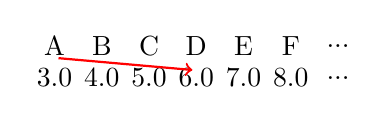
\begin{tikzpicture}[scale=0.5]
                    \foreach \x/\l in {0/A,1/B,2/C,3/D,4/E,5/F} {
                        \node at (\x*1.2, 0) {\l};
                        \node at (\x*1.2, -0.8) {\pgfmathparse{Mod(\x+3,26)}\pgfmathresult};
                    }
                    \node at (7.2, 0) {...};
                    \node at (7.2, -0.8) {...};
                    \draw[->, thick, red] (0.1,-0.3) -- (3.5,-0.6);
                \end{tikzpicture}
            \end{center}
        \end{column}
    \end{columns}
\end{frame}

\begin{frame}{Cifrul Vigenère}
    \begin{columns}
        \begin{column}{0.6\textwidth}
            \textbf{Principiu:}
            \begin{itemize}
                \item Cifru polialfabetic
                \item Folosește un cuvânt-cheie
                \item Fiecare literă din cheie determină shift-ul
            \end{itemize}

            \textbf{Exemplu:}
            \begin{center}
                \begin{tabular}{l|cccccccc}
                    Plaintext & A & T & T & A & C & K & A & T \\
                    \hline
                    Key & K & E & Y & K & E & Y & K & E \\
                    \hline
                    Shift & 10 & 4 & 24 & 10 & 4 & 24 & 10 & 4 \\
                    \hline
                    Ciphertext & K & X & R & K & G & I & K & X \\
                \end{tabular}
            \end{center}
        \end{column}
        \begin{column}{0.4\textwidth}
            \textbf{Avantaje vs Caesar:}
            \begin{itemize}
                \item Mai multe substituții
                \item Rezistă analiza simplă
            \end{itemize}

            \textbf{Vulnerabilități:}
            \begin{itemize}
                \item Testul Kasiski
                \item Testul Friedman
                \item Chei scurte = pattern-uri
            \end{itemize}
        \end{column}
    \end{columns}
\end{frame}

% ============================================================
\section{Criptare Modernă - AES}
% ============================================================

\begin{frame}{AES (Advanced Encryption Standard)}
    \begin{block}{Prezentare Generală}
        \begin{itemize}
            \item Standard NIST din 2001 (înlocuiește DES)
            \item Bazat pe algoritmul Rijndael
            \item Lungimi cheie: 128, 192, sau 256 biți
            \item Dimensiune bloc: 128 biți
        \end{itemize}
    \end{block}

    \begin{columns}
        \begin{column}{0.5\textwidth}
            \textbf{Structura unei runde:}
            \begin{enumerate}
                \item \textbf{SubBytes} - substituție neliniară (S-box)
                \item \textbf{ShiftRows} - permutare pe rânduri
                \item \textbf{MixColumns} - difuzie pe coloane
                \item \textbf{AddRoundKey} - XOR cu subcheia
            \end{enumerate}
        \end{column}
        \begin{column}{0.5\textwidth}
            \textbf{Număr de runde:}
            \begin{itemize}
                \item AES-128: 10 runde
                \item AES-192: 12 runde
                \item AES-256: 14 runde
            \end{itemize}

            \textbf{Moduri de operare:}
            \begin{itemize}
                \item ECB (nu se recomandă)
                \item \textbf{CBC} (folosit în proiect)
                \item CTR, GCM
            \end{itemize}
        \end{column}
    \end{columns}
\end{frame}

\begin{frame}{AES - Structura Rundei}
    \begin{center}
        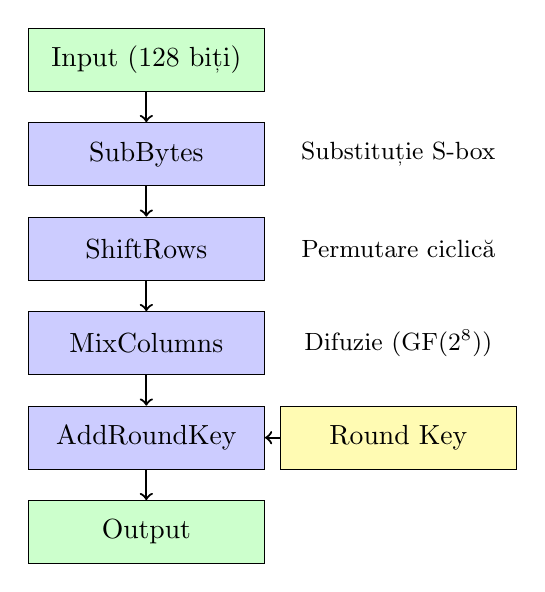
\begin{tikzpicture}[
            node distance=1.2cm,
            box/.style={draw, rectangle, minimum width=3cm, minimum height=0.8cm, fill=blue!20},
            arrow/.style={->, thick}
        ]
            \node[box, fill=green!20] (input) {Input (128 biți)};
            \node[box, below of=input] (sub) {SubBytes};
            \node[box, below of=sub] (shift) {ShiftRows};
            \node[box, below of=shift] (mix) {MixColumns};
            \node[box, below of=mix] (add) {AddRoundKey};
            \node[box, fill=green!20, below of=add] (output) {Output};
            \node[box, fill=yellow!30, right of=add, xshift=2cm] (key) {Round Key};

            \draw[arrow] (input) -- (sub);
            \draw[arrow] (sub) -- (shift);
            \draw[arrow] (shift) -- (mix);
            \draw[arrow] (mix) -- (add);
            \draw[arrow] (add) -- (output);
            \draw[arrow] (key) -- (add);

            % Annotations
            \node[right of=sub, xshift=2cm, font=\small] {Substituție S-box};
            \node[right of=shift, xshift=2cm, font=\small] {Permutare ciclică};
            \node[right of=mix, xshift=2cm, font=\small] {Difuzie (GF($2^8$))};
        \end{tikzpicture}
    \end{center}
\end{frame}

% ============================================================
\section{Funcții Hash}
% ============================================================

\begin{frame}{Funcții Hash Criptografice}
    \begin{block}{Definiție}
        O funcție hash $H$ transformă date de lungime arbitrară într-o amprentă de lungime fixă:
        $$H: \{0,1\}^* \rightarrow \{0,1\}^n$$
    \end{block}

    \textbf{Proprietăți esențiale:}
    \begin{enumerate}
        \item \textbf{Determinism}: același input $\Rightarrow$ același output
        \item \textbf{Eficiență}: calculul hash-ului este rapid
        \item \textbf{Preimage resistance}: dat $h$, imposibil de găsit $m$ a.î. $H(m) = h$
        \item \textbf{Second preimage resistance}: dat $m_1$, imposibil de găsit $m_2 \neq m_1$ a.î. $H(m_1) = H(m_2)$
        \item \textbf{Collision resistance}: imposibil de găsit $m_1 \neq m_2$ a.î. $H(m_1) = H(m_2)$
        \item \textbf{Efectul avalanșă}: mică schimbare în input $\Rightarrow$ hash complet diferit
    \end{enumerate}
\end{frame}

\begin{frame}{SHA-256 - Demonstrație Efectul Avalanșă}
    \begin{exampleblock}{Exemplu practic}
        \textbf{Input 1:} "Hello World"

        \textbf{Hash 1:} \texttt{a591a6d40bf420404a011733cfb7b190\\d62c65bf0bcda32b57b277d9ad9f146e}

        \vspace{0.3cm}
        \textbf{Input 2:} "Hello World!" (doar adăugat "!")

        \textbf{Hash 2:} \texttt{7f83b1657ff1fc53b92dc18148a1d65d\\fc2d4b1fa3d677284addd200126d9069}
    \end{exampleblock}

    \vspace{0.3cm}
    \begin{center}
        \textbf{Diferență: $\sim$50\% din biți sunt diferiți!}
    \end{center}

    \textbf{Utilizări:}
    \begin{multicols}{2}
        \begin{itemize}
            \item Verificarea integrității fișierelor
            \item Stocarea parolelor (cu salt)
            \item Semnături digitale
            \item Blockchain / Criptomonede
            \item Certificate digitale
            \item HMAC (autentificare mesaje)
        \end{itemize}
    \end{multicols}
\end{frame}

% ============================================================
\section{Demonstrație Aplicație}
% ============================================================

\begin{frame}{Arhitectura Aplicației}
    \begin{center}
        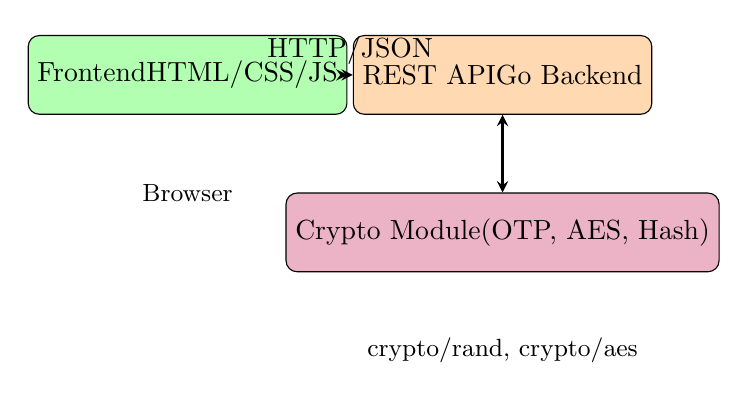
\begin{tikzpicture}[
            node distance=2cm,
            box/.style={draw, rectangle, rounded corners, minimum width=3cm, minimum height=1cm, fill=blue!20},
            arrow/.style={->, thick, >=stealth}
        ]
            \node[box, fill=green!30] (frontend) {Frontend\\HTML/CSS/JS};
            \node[box, fill=orange!30, right of=frontend, xshift=2cm] (api) {REST API\\Go Backend};
            \node[box, fill=purple!30, below of=api] (crypto) {Crypto Module\\(OTP, AES, Hash)};

            \draw[arrow, <->] (frontend) -- node[above] {HTTP/JSON} (api);
            \draw[arrow, <->] (api) -- (crypto);

            % Labels
            \node[below of=frontend, yshift=0.5cm, font=\small] {Browser};
            \node[below of=crypto, yshift=0.5cm, font=\small] {crypto/rand, crypto/aes};
        \end{tikzpicture}
    \end{center}

    \vspace{0.5cm}
    \textbf{Tehnologii folosite:}
    \begin{multicols}{2}
        \begin{itemize}
            \item \textbf{Backend:} Go (Golang)
            \item \textbf{Frontend:} HTML5, CSS3, JavaScript
            \item \textbf{Crypto:} crypto/rand, crypto/aes
            \item \textbf{API:} REST (JSON)
            \item \textbf{Hash:} Web Crypto API (client-side)
            \item \textbf{Docs:} LaTeX (Beamer + Article)
        \end{itemize}
    \end{multicols}
\end{frame}

\begin{frame}{Funcționalități Implementate}
    \begin{columns}
        \begin{column}{0.5\textwidth}
            \textbf{Algoritmi de Criptare:}
            \begin{enumerate}
                \item \textbf{OTP} (One-Time Pad)
                    \begin{itemize}
                        \item Generare cheie aleatorie
                        \item Criptare/Decriptare XOR
                        \item Demo key reuse attack
                    \end{itemize}
                \item \textbf{Caesar Cipher}
                    \begin{itemize}
                        \item Deplasare configurabilă
                        \item Atac brute-force
                    \end{itemize}
                \item \textbf{Vigenère Cipher}
                    \begin{itemize}
                        \item Cuvânt-cheie
                        \item Tabelă interactivă
                    \end{itemize}
            \end{enumerate}
        \end{column}
        \begin{column}{0.5\textwidth}
            \textbf{Criptare Modernă:}
            \begin{enumerate}
                \setcounter{enumi}{3}
                \item \textbf{AES-256}
                    \begin{itemize}
                        \item Mod CBC
                        \item Padding PKCS7
                        \item IV aleatoriu
                    \end{itemize}
                \item \textbf{SHA-256 Hash}
                    \begin{itemize}
                        \item Hashing în timp real
                        \item Demo efect avalanșă
                    \end{itemize}
            \end{enumerate}

            \vspace{0.5cm}
            \textbf{Interfață:}
            \begin{itemize}
                \item Design modern, responsive
                \item Explicații teoretice
                \item Vizualizări interactive
            \end{itemize}
        \end{column}
    \end{columns}
\end{frame}

% ============================================================
\section{Concluzii}
% ============================================================

\begin{frame}{Comparație Algoritmi}
    \begin{center}
        \begin{tabular}{|l|c|c|c|c|}
            \hline
            \textbf{Algoritm} & \textbf{Tip} & \textbf{Securitate} & \textbf{Practică} & \textbf{Utilizare} \\
            \hline
            OTP & Simetric & Perfectă & Limitată & Militar \\
            \hline
            Caesar & Substituție & Foarte slabă & Nu & Educațional \\
            \hline
            Vigenère & Polialfabetic & Slabă & Nu & Educațional \\
            \hline
            AES-256 & Simetric (bloc) & Foarte puternică & Da & Standard \\
            \hline
            SHA-256 & Hash & Puternică & Da & Integritate \\
            \hline
        \end{tabular}
    \end{center}

    \vspace{0.5cm}
    \begin{block}{Lecții învățate}
        \begin{itemize}
            \item OTP oferă securitate perfectă teoretic, dar e impractică
            \item AES este standardul de facto pentru criptare simetrică
            \item Funcțiile hash sunt esențiale pentru integritate și autentificare
            \item Securitatea depinde de implementare, nu doar de algoritm
        \end{itemize}
    \end{block}
\end{frame}

\begin{frame}{Concluzii și Recomandări}
    \textbf{Ce am realizat:}
    \begin{itemize}
        \item Aplicație web demonstrativă pentru algoritmi criptografici
        \item Implementare corectă în Go folosind biblioteci standard
        \item Documentație completă și prezentare
    \end{itemize}

    \vspace{0.3cm}
    \textbf{Recomandări pentru practică:}
    \begin{enumerate}
        \item \textbf{Nu implementați propriii algoritmi} - folosiți biblioteci testate
        \item \textbf{Alegeți algoritmi moderni}: AES-256, SHA-256/SHA-3, ChaCha20
        \item \textbf{Generare chei securizată}: crypto/rand, nu math/rand
        \item \textbf{Nu reutilizați cheile} (mai ales pentru OTP)
        \item \textbf{Folosiți moduri sigure}: GCM pentru autentificare
    \end{enumerate}

    \vspace{0.3cm}
    \begin{alertblock}{Principiu de aur}
        \textbf{"Don't roll your own crypto"} - Bruce Schneier
    \end{alertblock}
\end{frame}

\begin{frame}{Resurse și Referințe}
    \textbf{Bibliografie:}
    \begin{itemize}
        \item Shannon, C. E. (1949). "Communication Theory of Secrecy Systems"
        \item Schneier, B. (2015). "Applied Cryptography"
        \item Ferguson, N., Schneier, B. (2010). "Cryptography Engineering"
        \item NIST FIPS 197 - AES Standard
    \end{itemize}

    \vspace{0.5cm}
    \textbf{Resurse online:}
    \begin{itemize}
        \item Go Crypto Package: \url{https://pkg.go.dev/crypto}
        \item OWASP Cryptographic Guidelines
        \item CrypTool - Instrument educațional
    \end{itemize}

    \vspace{0.5cm}
    \begin{center}
        \textbf{Mulțumesc pentru atenție!}

        \textbf{Întrebări?}
    \end{center}
\end{frame}

\end{document}
